% Styling and set-up
\documentclass{article}


\usepackage{NotesStyle}
\graphicspath{./figs/}

% Cover info

\title{Phys 514 \\
	\large Relativity}

\author{April Sada Solomon}
\date{Winter 2021}


% Document
\begin{document}

	\clearpage
	% Displays title info
	\maketitle
	
	\vspace{2cm}
	
	% Course description, displayed on cover page
	\renewcommand{\abstractname}{Course Description}
	\begin{abstract}
		 Notes taken directly from the lectures given by Dr. Maloney (not proof read by him). Special Relativity, Manifolds, Spacetime Curvature, Gravitation, Schwarzchild Solution, Black Holes, Perturbations, Radiation, Introduction to Cosmology, Introduction to QFT in Spacetime. 
	\end{abstract}
	
	\newpage
	
	\tableofcontents
	
	\newpage
	
	% Start page count after the TOC
	\setcounter{page}{1}
	\cfoot{\thepage}
	
	% Notes body
	\section{A Brief Review of Special Relativity}
	\subsection{Introduction}
 		General Relativity is the modern theory of classical gravity. What do we mean by "classical"? Simply, it is a nomenclature to distinguish from Quantum Mechanics, so those effects are ignored. The basic idea from Newtonian Mechanics is that gravity is a force, and as we know, most forces are described by fields.
 		
 		The simplest example of a field that describes a force is the Newtonian gravitational potential $\Phi (\vec{r})$:
 		\begin{equation}
 			\label{eq:NetwonGravitation}
 			\frac{d}{dt}\frac{\partial \Lgr}{\partial \dot{x}} = \frac{\partial \Lgr}{\partial x} \implies \vec{F} (\vec{v}) = - \frac{\partial}{\partial \vec{r}} \Phi (\vec{r}) 
 		\end{equation}
 		\noindent
 		If we are studying electromagnetism, we would study the electromagnetic fields $\vec{E}$ and $\vec{B}$. Let us list the Maxwell Equations, that we will review again later on:
 			\begin{align}
 				\label{eq:Maxwell}
 				\grad \cdot \vec{E} &= \frac{\rho}{\varepsilon_0} \\
 				\grad \cdot \vec{B} &= 0 \\
 				\grad \times \vec{E} &= -\frac{\partial \vec{B}}{\partial t} \\
 				\grad \times \vec{B} &= \mu_0 \left( \vec{J} + \varepsilon_0 \frac{\partial \vec{E}}{\partial t} \right)
 			\end{align}
 		A classical field theory like the theory of Newtonian gravity or the theory of Electromagnetism has two parts that describe it:
 		\begin{enumerate}
 			\item \textbf{Field equation}
 				\subitem A field equation is an equation of motion that describes exactly how a certain field is determined by some set of sources. In other words, it is usually a second order differential equation that has to be solved to determine the field from some collection of sources. 
 			\begin{exmp}
 				Newtonian gravity field equation
 				$$ \nabla^2 \Phi = 4\pi G \rho$$
 				where $\rho$ is the mass density. We solve this Laplace's equation to determine the field. If $\rho$ is a $\grad(\vec{r})$ function such that it describes a point mass, which implies that
 				$\Phi \propto \nicefrac{1}{\vec{r}}$.
 			\end{exmp}
	 		\begin{exmp}
	 			Electromagnetic field equations. See the \hyperref[eq:Maxwell]{Maxwell's Equation's} above. In equation (1.2), we have that $\rho$ represents the charge density to determine the field in terms of the forces from some collection of charge sources.
	 		\end{exmp}
 		\pagebreak
 			\item \textbf{Force law}
 			\subitem The force law is an equation that determines how an object moves in the presence of a field. So we start by describing a collection of sources and how they describe some force field, and then we use the force law to determine how bodies in motion are affected by the force field using the force law.
 			\begin{exmp}
 				Newtonian force law
 				$$ \vec{F}(t, \vec{x}, \dot{\vec{x}}) = \frac{m}{2}\frac{d}{dt} \frac{\partial}{\partial \vec{v}}\vec{v}^2 = m \dot{\vec{v}} =- m \vec{\grad} \Phi(t,\vec{x}) $$
 				where $\dot{\vec{v}} = \nicefrac{d^2 \vec{x}}{dt^2} = \ddot{\vec{x}}$. This force law describes how some gravitational potential affects the motion of bodies in the presence of the field described by the potential.
 			\end{exmp}
 			\begin{exmp}
 				Lorentzian force law
 				$$ \vec{F} \left(t, \vec{x}, \dot{\vec{x}}\right)=q (\vec{E} + \vec{v} \times \vec{B} )$$
 				where $\vec{v} = \nicefrac{d\vec{x}}{dt} = \dot{\vec{x}}$.
 			\end{exmp}
 			The important thing here is that fields are just functions of points in spacetime. For example, the gravitational potential $\Phi (t, \vec{x})$ yields a number that depends on where you are in space time, and the electric field $\vec{E} (t, \vec{x})$ is also a vector that depends on where you are in space and time. We should think of force laws as equations that describe how the motion of objects deviate from being "straight lines". 
 		\end{enumerate}
 		To emphasize, let us assume that an object in inertial motion on the $+\hat{x}$ axis, neglecting field interactions with the object. Evidently so, it's acceleration is zero, yielding the differential equation $\ddot{x} = 0$. The solution to this second order differential equation yields motion in a straight line. So the force law considering a field with an object experiencing this motion will be able to distort the object's motion such that it is not a straight line anymore. For instance, a gravitational field will bend the straight line into a curve as it generates acceleration in the $-\hat{y}$ axis, leading to parabolic motion on the $\hat{x}\hat{y}-$plane.
 		
 		\begin{defn}
 			\textbf{General Relativity} is a complete reinterpretation of gravitation such that it is not a field using a potential $\Phi (t, \vec{x})$, but instead it is a feature of spacetime itself. In particular, we replace the gravitational potential with a \textit{metric tensor} that describes this feature, particularly, the geometrical curvature of spacetime.
 		\end{defn} 
 		We will be learning pseudo-Riemann topological spaces by employing Einstein's field equation, which determines how spacetime curvature is determined in the presence of matter or energy. In Newtonian gravitation, the source term was a mass (or energy density in Special Relativity where $E = mc^2$). Recall however that mass has no independent meaning in terms of relativity as energy and momentum both depend on the reference frame where they are measured. The "source" of the curvature in general relativity is a term in the Einstein field equations that describes a generalized mass-energy distribution in spacetime of the sources present.
 		
 		The force law is also replaced by the geodesic equation, which tells us how objects move through some curved spacetime. Particularly, the geometric interpretation of the geodesic is quite simple; it is the statement that \textit{object will move on \textbf{geodesics}, which are the shortest paths between two points on a surface.} In a flat surface, this is a straight line, but in curved surfaces, this trajectory will not be a straight line, like two points on the surface of a sphere.
 		
 		\begin{figure}[h]
 			\begin{subfigure}{0.46\textwidth}
 				\center
 				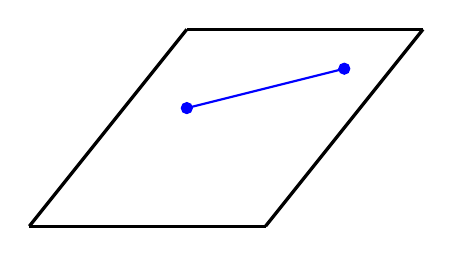
\begin{tikzpicture}
 					\draw [very thick] (-1,-2) -- (1,0.5);
 					\draw [very thick] (2,-2) -- (4,0.5);
 					\draw [very thick] (-1,-2) -- (2,-2);
 					\draw [very thick] (1,0.5) -- (4,0.5);
 					
 					\draw [thick, blue] (1, -0.5) -- (3, 0);
 					
 					\filldraw [blue] (1, -0.5) circle (2pt)
 					(3,0) circle (2pt);
 				\end{tikzpicture}
 			\vspace{0.5cm}
 			\caption{Geodesic over a flat surface}
 			\end{subfigure}
 			\begin{subfigure}{0.46\textwidth}
 				\center
 				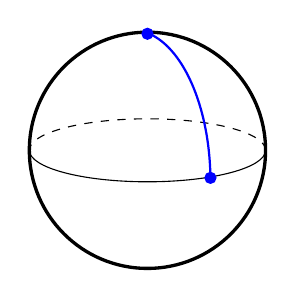
\begin{tikzpicture}
 					\draw [very thick] (0,0) circle (1.5cm);
 					\draw [dashed] (1.5,0) arc (0:180:1.5 and 0.4);
 					\draw (1.5,0) arc (0:180:1.5 and -0.4);
 					
 					\draw [thick, blue] (0.8, -0.35) arc (1.5:80:1 and 1.93);
 					
 					\filldraw [blue] (0.8,-0.35) circle (2pt)
 					(0,1.48) circle (2pt);
 				\end{tikzpicture}
 				\caption{Geodesic over a spherical surface}
 			\end{subfigure}
 			\caption{Examples of geodesic on different surfaces.}
 		\end{figure}
 		So in other words, it is the curve that minimizes the distance between two points over some surface. The force law is therefore just the statement that bodies will move in geodesics over some geometry, even when said geometry is curved. So when we think of gravity as the curvature of spacetime, then geodesics will describe motion over spacetime as it is curved.
 		
 		\subsection{Special Relativity}
 		The discussion of special relativity will serve to introduce spacetime properly. We will develop it further later on, but for now we will proceed with a heuristic manner. 
 		
 		\begin{defn}
 			\textbf{Spacetime} is a smoothly connected manifold where the points defined are called \textbf{events}.
 		\end{defn}
 		The events in spacetime can be smoothly parametrized using coordinates, such as the most common system of coordinates used, the Cartesian coordinates.
 		\begin{exmp}
 			Cartesian coordinates
 			$$ (t, \vec{x}) = (-c\hat{t}, \hat{x}, \hat{y}, \hat{z})$$
 			In relativistic mechanics, we usually consider all directions of motion in a single vector $\vec{x} = (\hat{x}, \hat{y}, \hat{z})$ while time is multiplied by the negative speed of light $t = (-c\hat{t})$. We will explain this later on.
 		\end{exmp}
 		Thus, spacetime is a smooth manifold with events as points parametrized by some coordinates, and in relativity, we know that physics should be independent of its coordinate system. This is known as the \textbf{principle of general covariance}.
 		
 		\pagebreak
 		To begin, let us assume we are working with Newtonian mechanics where we have two points in spacetime labelled $(t_1, \vec{x}_1) = (t_1, x_1, y_1, z_1)$ and $(t_2, \vec{x}_2) = (t_2, x_2, y_2, z_2)$ respectively, both of which describe a single event in spacetime given as $$(\Delta t, \Delta \vec{x})$$ 
 		In this event, $\Delta t$ denotes the \textbf{temporal separation} while $\Delta \vec{x}$ denotes the \textbf{spatial separation}. Explicitly:
 		\begin{align*}
 			\Delta t &=	t_2 - t_1\\
 			\Delta \vec{x} &= \sqrt{(\vec{x}_2 - \vec{x}_1)\cdot (\vec{x}_2 - \vec{x}_1)}\\ 
 			&= \sqrt{(x_2 - x_1)^2 + (y_2 - y_1)^2 + (z_2 - z_1)^2} & (\text{in Cartesian coordinates})
 		\end{align*}
 		This makes sense as Newtonian mechanics can always be written in terms of both $\Delta t$ and $\Delta \vec{x}$, so the numerical value of $t_1$ will depend on the origin in the frame of reference we are working on. In other words, if we choose our reference frame to be Montreal at 6:00pm and remain at rest until 6:01pm, then we can denote that $\Delta t = 60$ s. So if we now jog in Montreal at constant velocity of $1$ m/s in this reference frame, the velocity will depend on the time separation $\Delta t$ and not on the absolute values of $t_1$ and $t_2$. So, if we suddenly change the time frame to be 4:20pm to 4:21pm, the velocity should not vary due to the absolute value of the new points in time, as the time separation $\Delta t$ would be the equal to the case at 6:00pm. The same would go for the choice of spatial coordinates, so if we move from Montreal to Toronto and the speed remains constant, the space separation $\Delta \vec{x}$ should also not vary. To summarize, the laws of physics would remain invariant even if we change the choice of reference frame where the choice of time is independent of the choice of space, and so they are independent of the entire coordinate system chosen. Albeit elementary to classical mechanics, it is vital to understand this properly to proceed with the philosophy of relativity.
 		
 		In special relativity, there is no separate notion between space and time, so we denote both as spacetime. This means that the both the separation of time and the separation of space are dependent on each other, which leads to effects like time dilation. Time dilation implies that \textit{the temporal difference $\Delta t$ of two event in spacetime will depend on the relative position in spacetime where an observer is viewing the event from}. Similarly, the distance or length of an object will depend on where the observer is in spacetime. In other words, we cannot think of $\Delta t$ and $\Delta \vec{x}$ as independent separations in spacetime, as one is directly related to the other depending on the frame of reference. So, observing the same event in a different reference frame will change the values of $\Delta t$ and $\Delta \vec{x}$. 
 		
 		However, we can denote an invariant notion to both the spatial and temporal separations called the \textbf{interval} between two events as
 		$$ \Delta s^2 = -c^2 \Delta t^2 + \Delta \vec{x}^2 \quad \quad (\text{in Cartesian coordinates})$$
 		Usually, we simplify by allowing $c=1$ in units in terms of the speed of light [$3\times 10^8$ m/s] such that
 		\begin{equation}
 			\label{eq:Interval}
 			\Delta s^2 = - \Delta t^2 + \Delta \vec{x}^2
 		\end{equation}
 		So when we measure distance with respect to the speed of light, we do so in terms of light-time, such as light-seconds and light-years. It is usually helpful to draw pictures in a spacetime diagram.
 		\begin{figure}[h]
 			\center
 			\begin{tikzpicture}[scale=1.6]
 				% Grid
 				\filldraw [green, opacity=0.25] (-3, 1) -- (-3, 3) -- (3,3) -- (3,2) -- (-0.5, -1.5);
 				\filldraw [green, opacity=0.25] (-1, -2) -- (-0.5, -1.5) -- (0,-2);
 				\filldraw [red, opacity=0.1] (-3,1) -- (-0.5, -1.5) -- (-1, -2) -- (-3, -2);
 				\filldraw [red, opacity=0.1] (3,2) -- (-0.5, -1.5) -- (0, -2) -- (3, -2);
 				\draw [step=0.5cm, grey, opacity=0.25] (-3,-2) grid (3,3);
 				% Axes
 				\draw [->, thick, >=stealth] (-0.5, -2) -- (-0.5, 2.5)
 				node [above] {$t$};
 				\draw [->, thick, >=stealth] (-3, -1.5) -- (2.5, -1.5)
 				node [right] {$x$};
 				\draw [->, thick,blue, >=stealth] (-0.62, -2) -- (0.5, 2.5)
 				node [above] {$t'$};
 				\draw [->, thick, blue, >=stealth] (-1.95, -2) -- (2.5, -0.5)
 				node [right] {$x'$};
 				% Light cone
 				\draw [green] (1.5, 2.85) node [] {Time-like, $s^2 < 0$} (1.5, 2.65) node [] {Future} (-0.33, -1.88) node [] {\smaller Past} ;
 				\draw [red] (2.5, 0) node [] {Space-like} (2.5,-0.23) node [] {$s^2 > 0$};
 				\draw [black] (2 , 1.3) node [] {\small$x = t$}
 				(-1.5,0)node [] {\small$x = -t$}
 				;
 				\draw [blue] (2.5 , 1) node [] {\small$x' = t'$}
 				(-2,-0.5)node [] {\small$x' = -t$}
 				;
 				\draw [very thick, olive] (-1, -2) -- (3, 2)
 				;
 				\draw [very thick, olive] (-3, 1) -- (0, -2);
 				% Event is the same
 				\draw [dashed] (-0.5, 1.5) -- (1.5, 1.5);
 				\draw [dashed] (1.5, -1.5) -- (1.5, 1.5);
 				\draw [dotted, thick, blue] (0.21, 1.2) -- (1.5, 1.5);
 				\draw [dotted, thick, blue] (0.7, -1.08) -- (1.5, 1.5);
 				\filldraw [black] (1.5, 1.5) circle (1.5pt) node [above=2mm] {\small Event}; 
 				
 			\end{tikzpicture}
 		\caption{A spacetime diagram of an time-like event with the light cone in two different reference frames, a static frame $K= (t,x)$ and another moving away from the static frame at a fraction of the speed of light, $K' = (t', x')$. Notice how even if the spatial ($\Delta x \neq \Delta x'$) and temporal ($\Delta t \neq \Delta t'$) separations vary from one reference frame to the other, the interval in spacetime remains invariant $\Delta s^2 = \Delta(s')^2$. We usually denote $(t_1, x_1) = (t_1', x_1') = (0,0)$ for convenience in either reference frame.}
 		\end{figure}
 	
 		Notice in the spacetime diagram that when $\Delta s^2 = 0$, we have that $\Delta x = \pm \Delta t$, defining a \textbf{light cone}. Events defined on the light cone are denoted \textbf{light-separated events} or \textbf{null-separated events}. As otherwise noted, events where $\Delta s^2 < 0 $ are inside the light cone and denoted as \textbf{time-like} or \textbf{time-separated}, while events where $\Delta s^2 > 0$ lie outside the light cone and are denoted as \textbf{space-like} or \textbf{space-separated}. Notice that for time-like events, it is clear that when $t_2 > 0$, the event will propagate to the future, while if $t_2 < 0$ it propagates to the past. Also note that space-like events are deemed as impossible, as there is no geodesic inside a light cone that can connect the origin to the event. In other words, an object would have to travel faster than light to arrive at this location in spacetime, which is indeed impossible in special relativity.
 		
 		We can thus assume that if we fix $\Delta s^2$ in a spacetime phase for the system
 		\vspace{0.5cm}
 		$$ \begin{pmatrix}
 			\nicefrac{\partial \left( \Delta \vec{x}^2 \right)}{\partial\left( \Delta s^2 \right)} \\
 			\nicefrac{\partial \left( \Delta t^2 \right)}{\partial\left( \Delta s^2 \right)}
 		\end{pmatrix}=\begin{pmatrix}
 			0 & \pm1 \\
 			\pm 1 & 0
 		\end{pmatrix} \begin{pmatrix}
 		\Delta \vec{x}^2 \\
 		\Delta t^2
 		\end{pmatrix}$$
 	
 		\pagebreak \noindent
 		We would get hyperbolic equilibrium to a 2D spacetime system with respect to the interval $\Delta s^2$. This means a time-like event will always be either time-like or get close to null-like, while a space-like event will also either remain space-like or get close to null-like. 
 	
 		\begin{claim}
 			We can reduce Special Relativity to the statement that for 2 time-like separated events, the proper time $\Delta \tau$ measured by an observer moving at constant velocity between the two events is given by:
 			$$ \left( \Delta \tau \right)^2  = - \left( \Delta s \right)^2$$
 		\end{claim}
 		
 		\begin{exmp}
 			\textbf{Time dilation}
 			\begin{figure}[h]
 				\begin{minipage}{0.4\textwidth}
 					\center
 					\begin{tikzpicture}[scale=1]
 						%\draw (2,2) node []{$\M$} ;
 						\draw [step=0.5cm, grey, opacity=0.25] (-2.5,-2.5) grid (2.5,2.5);
 						\draw [->, very thick,  blue, >=stealth] (-1,-2) -- (-1,1.95);
 						\draw [->, very thick, green, >=stealth] (-1,-2) -- (0.5,-0.05);
 						\draw [->, very thick, green, >=stealth] (0.5,0) -- (-0.95,1.95);
 						\draw [->] (-2, -2.5) -- (-2, 2) node (taxis) [above] {$t$};
 						\draw [->] (-2.5, -2) -- (2, -2) node (xaxis) [right] {$x$};
 						\filldraw (-1, -2) circle (2pt) node [right =2mm, below] {$A$}
 						(-1, 2 ) circle (2pt) node [right =2mm, above] {$C$}
 						(-1, 0) circle (2pt) node [right =2mm, below] {$B$}
 						(0.5, 0) circle (2pt) node [right =2mm, below] {$B'$};
 						\draw [<->, blue] (-1.5, -2) -- (-1.5, 2) node [left=2mm, below=1.9cm] {$\Delta t$};
 						\draw [<->, green, >=stealth] (-0.95, 0) -- (0.45, 0) node [left=0.8cm, above=-0.2mm] {$\Delta x$};
 					\end{tikzpicture}
 					\caption{Spacetime diagram for the twin's paradox. Notice that the inclination of the trajectory of the second twin is greater than $\nicefrac\pi4$ with respect to the $x$-axis, implying that the speed $v<c$.}
 				\end{minipage}
 				\hfill
 				\begin{minipage}{0.56\textwidth}
 					\begin{spacing}{1.5}
 						Here, we see the famous \textit{twin's paradox}. We have two observers relative to a frame of reference, usually considered twins, that will go from a point $A(t,x) = (0, 0)$ to a point $C(t,x)=(\Delta t, 0)$ in spacetime. The first twin will remain static in space while the second will go to point $B' (t,x) = \left(\frac{\Delta t}{2}, \Delta x\right)$ before reaching point $C$, where $\Delta x = \frac12 v \Delta t$ for constant propagation velocity $v$. The proper time for the trajectory of the first twin from $A$ to $B$ is clearly $\tau_{B,A} = \frac{\Delta t}{2}$, but for the second twin, the proper time from $A$ to $B'$ is given by
 					\end{spacing}
 				\end{minipage}
 			\end{figure} 
 			\vspace{-0.5cm}
 			$$ \tau_{B',A}^2 = \left(\frac{\Delta t}{2}\right)^2 - (\Delta x)^2 $$
 			\begin{equation}
 				\label{eq:RelativeProperTime}
 				\therefore \boxed{\tau_{B',A} = \frac{\Delta t}{2} \sqrt{1 - v^2} }
 			\end{equation}
 			
 			By symmetry, it follows that $\tau_{C,B} = \tau_{B,A}$ and $\tau_{B', A} = \tau_{C, B'}$. Considering the entire sequence of movement for both twins, we have
 			\begin{align*}
 				\tau_{C,B,A} &= \Delta t \\
 				\tau_{C,B',A} &= \sqrt{1 - v^2} \Delta t
 			\end{align*}
 			Clearly, $\tau_{C,B,A} > \tau_{C,B',A}$, and so the second twin is younger than the first twin by the time they both reach the point $C$. This implies that the proper time $\tau$ along some world line is related to the interval $\Delta s^2$ traversed through spacetime. Therefore, we can assess the ratio of relative time difference between the twins as 
 			$$ \frac{2 \tau_{C,B',A}}{\tau_{C,B,A}} = \sqrt{1-v^2} $$
 		\end{exmp}
 	\pagebreak
 		\begin{exmp}
 			\textbf{Length contraction} 
 			\begin{figure}[h]
 				\begin{minipage}{0.4\textwidth}
 					\center
 					\begin{tikzpicture}[scale=1]
 						%\draw (2,2) node []{$\M$} ;
 						\draw [step=0.5cm, grey, opacity=0.25] (-2.5,-2.5) grid (2.5,2.5);
 						
 						\draw [->] (-2, -2.5) -- (-2, 2) node (taxis) [above] {$t$};
 						\draw [->] (-2.5, -2) -- (2, -2) node (xaxis) [right] {$x$};
 						
 						\draw [->, very thick, blue,>=stealth] (-2,-2) -- (-1, 2)
 						 node [left=9mm, below=10mm] {$x=vt$};
 						\draw [->, very thick, green, >=stealth] (-2,-2) -- (0.5, 0.5)
 						 node [left=13mm, below=5mm] {$x=t$};
 						\draw [->, very thick, green, >=stealth] (0.5, 0.5) -- (-1,2)
 						 node [right=12mm, below=0mm] {$x=2L-t$};
 						
 						\draw [very thick] (0.5, -2) -- (0.5, 2.5);
 						\draw [very thick, red] (-2, -2) -- (0.5, -2);
 						\filldraw [red] (-2,-2) circle (1pt) node [below=3mm, right] {$(0,0)$}
 						(0.5, -2) circle (1pt) node [below] {$(0,L)$};
 						\filldraw [green] (0.5, 0.5) circle (1.5pt) node [right] {$(L,L)$};
 						\filldraw [black] (-1, 2) circle (1.5pt) node [above] {$(t_2, x_2)$};
 					\end{tikzpicture}
 					\caption{The spacetime diagram for length contraction. }
 				\end{minipage}
 				\hfill
 				\begin{minipage}{0.56\textwidth}
 					\begin{spacing}{1.5}
 						Consider an observer moving at constant velocity $v$ from the origin of a reference frame  with respect to a static ruler with a light bulb at the point $(0,0)$. We would like for the observer to measure the ruler using light-travel time, which is achieved by flashing the light bulb and measuring the time it takes to reach a point $(L,L)$, and return to the observer at the intersection point $(t_2, x_2)$. Noting how we have two solutions for $x$, namely $x = 2L-t$ and $x=vt$, we can equate them to find $(t_2, x_2)$ such that
 					\end{spacing}
 				\end{minipage}
 			\end{figure} 
 			\vspace{-1cm}
 			\begin{align*}
 				t_2 &= \frac{2L}{(1+v)}\\
 				x_2 &= v \left( \frac{2L}{(1+v)} \right)
 			\end{align*}
 			And so, the proper time $\Delta \tau^2$ measured by the observer at the point when the light bulb's ray is reflected back is given by $\Delta \tau^2 = \Delta t^2 - \Delta x^2$ such that
 			$$ \Delta \tau^2 = \left(\frac{2L}{(1+v)}\right)^2(1 - v^2)$$
 			Knowing that an observer at rest with the ruler $\Delta t^2$ for the light to reflect back on itself is $\Delta t = \frac{2L}{(1+v)}$, we get the ratio
 			$$ \frac{\Delta \tau^2}{\Delta t^2} = (1-v^2)$$
 			So the apparent length of the ruler would be shorter by a factor of $v^2$. Note that in the case where $x = -vt$ for the observer's trajectory, the same ratio would arise.
 		\end{exmp}
	 	We are very habituated to writing the interval in the following way
	 	$$ \Delta s^2 = - \Delta t^2 + \Delta x_1^2 + \Delta x_2^2 + \Delta x_3^2$$
	 	We will consider the $x^\mu$ notation, where $\mu=0,1,2,3$, to denote these coordinates as a single coordinate. Moreover, we can denote $x^i$ where $i=1,2,3$ as the spatial coordinates. Therefore, we may define
	 	\begin{multicols}{4}
	 		\begin{itemize}
	 			\item $x^0 = t$
	 			\item $x^2 = x_2$
	 			\item $x^1 = x_1$
	 			\item $x^3 = x_3$
	 		\end{itemize}
	 	\end{multicols}
	 	We can thus summarize the coordinates of some interval to a summation
	 	$$ \Delta s^2 = \sum_{\mu=\nu} \eta_{\nu\mu}\Delta x^\mu \Delta x^\nu$$ 
	 	Where we define $\eta_{\mu\nu}$ to be a $4\times4$ diagonal matrix such that
	 	$$ \eta_{\mu\nu} = \begin{pmatrix}
	 		-1	&	0	&	0	&	0\\
	 		0	&	1	&	0	&	0\\
	 		0	&	0	&	1	&	0\\
	 		0	&	0	&	0	&	1
	 	\end{pmatrix}$$ 
	 	\begin{defn}
	 		The \textbf{metric} of flat spacetime in Cartesian coordinates is given by the $4 \times 4$ matrix $\eta_{\mu\nu}$.
	 	\end{defn}
	 	We may further simplify the interval by using \textit{Einstein summation notation}. This notation takes the summation symbol for granted, which adds all terms in the resulting $4\times4$ matrix whose indices follow the property $\mu=\nu$, to get
 		\begin{equation}
 			\label{eq:IntervalEinstein}
 			\Delta s^2 = \eta_{\mu\nu} \Delta x^\mu \Delta x^\nu
 		\end{equation}
 		As such, in tensor calculus language this implies that for every subscript in a tensor we must have a corresponding superscript to yield an interval as desired. In this case, $\eta_{\mu\nu}$ has two subscripts, each denoting an index for the matrix, and the one-forms $\Delta x^\mu$ and $\Delta x^\nu$ each have one superscript to indicate their respective components. Hence, we can summarize special relativity to the statement that all intervals in spacetime can be given by an equation in the form of (\ref{eq:IntervalEinstein}), such that spacetime is denoted as \textbf{Minkowski spacetime} $\R^{1,3}$ or simply $\M$. To summarize for now, general relativity implies that spacetime can be something other than Minkowski spacetime $\M$.
 		
 		Other examples of spaces are Euclidean spaces, both in 2D ($\R^2$) and in 3D ($\R^3$), where an invariant interval is simply denoted as the distance between two points. Using the notation we have established, the coordinates in 2D and 3D respectively would be:
 		\begin{align*}
 			(x^1, x^2) &= (x,y) \\
 			(x^1, x^2, x^3) &= (x,y,z)
 		\end{align*}
 		For either of these, the distance is obtained by use of Pythagoras's theorem $D = \sqrt{(x^1)^2 + (x^2)^2 + (x^3)^3}$, where in 2D we simply neglect the $x^3$ term. Recall than an invariant interval is similarly given by $\Delta s^2 = -(x^0)^2 + (x^1)^2 + (x^2)^2 + (x^3)^3$.
 		where the $x^0$ term is given a negative sign. Note that an opposite yet equally valid for the invariant interval is $\Delta s^2 = \Delta t^2 - \Delta x^2 $. This convention is better for events happening in the same spatial coordinate at different points in time, while the one we used is better for events that happen at the same time in different spatial coordinates.
 		\begin{exe}
 			Recalling that a Lorentzian transformation $\Lambda$ is a linear change of coordinates, determine the correct form of the $2 \times 2$ matrix $\Lambda$ that validates the following change of coordinates:
 			$$ \begin{bsmallmatrix}
 				x \\
 				t
 			\end{bsmallmatrix} \to \begin{bsmallmatrix}
 			x' \\
 			t'
 			\end{bsmallmatrix} = \Lambda \begin{bsmallmatrix}
 			x\\t
 		\end{bsmallmatrix}$$
 		\end{exe}
 		
 		To summarize, the proper time $\Delta \tau$ measured by an observer moving at some constant velocity $v$ between two points in spacetime is given by
 		$$ (\Delta \tau)^2 = - (\Delta s)^2 = \Delta t^2 - \Delta \vec{x}^2$$
 		Where we could write the invariant interval $\Delta s^2$ using Einstein summation notation as 
 		$$ \Delta s^2 = \eta_{\mu\nu} \Delta x^\mu \Delta x^\nu$$
 		For the coordinates $\Delta x^\mu = (\Delta t, \Delta \vec{x})$ where $\mu = 0,1,2,3$, and the metric $\eta_{\mu\nu}$. Recall that this notation neglects a summation symbol that will sum all elements in the $4\times4$ matrix $\eta_{\mu\nu} \Delta x^\mu \Delta x^\nu$ that follow the property $\mu = \nu$.
 		
 		Thus far, we have only considered an observer moving at constant velocity for the sake of conceptual simplicity. However, when consider gravitation we will encounter accelerating reference frames. That is, we will encounter motion in spacetime that is not given by a straight line, but rather by some curve, implying variable velocity. 
 		\begin{defn}
 			A general path through spacetime is denoted as a \textbf{worldline} and can be parametrized with 4 functions, one for each coordinate in the metric.
 		\end{defn}
 		\begin{figure}[h]
 			\begin{minipage}{0.4\textwidth}
 				\center
 				\begin{tikzpicture}[scale=1]
 					%\draw (2,2) node []{$\M$} ;
 					\draw [step=0.5cm, grey, opacity=0.25] (-2.5,-2.5) grid (2.5,2.5);
 					
 					\draw [->] (-2, -2.5) -- (-2, 2) node (taxis) [above] {$t$};
 					\draw [->] (-2.5, -2) -- (2, -2) node (xaxis) [right] {$x$};
 					\draw [thick, dashed, green] (-2,-2) -- (2.5, 2.5) node [below=20mm, left=5mm] {$\Delta s^2 = 0$};
 					 
 					\draw [thick, blue] plot [smooth] coordinates{(-2,-2) (-1, -0.5) (-1, 0) (0, 0.5) (-0.5, 1) (1, 1.5)};
 					\draw [line width=0.6mm, red] plot [smooth] coordinates{(-0.05, 0.45) (0, 0.5) (-0.05, 0.6)} 
 					node [right] {ds};
 					
 					
 					\filldraw (-2, -2) circle (2pt) (1,1.5) circle (2pt);
 				\end{tikzpicture}
 				\caption{A worldline in spacetime of a time-like observer accelerating, with a line element shown. Notice how at every point on the worldline, the observer's speed has the property $v<c$.}
 			\end{minipage}
 			\hfill
 			\begin{minipage}{0.56\textwidth}
 				\begin{spacing}{1.5}
 					The parametrization in Cartesian coordinates for a worldline using $\lambda$ as the variable which denotes points along the world line is as follows:
 					$$ x^\mu (\lambda) = \left(t(\lambda), x^1 (\lambda), x^2(\lambda), x^2 (\lambda)\right)$$
 					Along this worldline, we consider infinitesimally small displacements through space $d\vec{x}$ and through time $dt$ such that at each interval of displacement we approximate to constant velocity. The proper time $\Delta \tau$ measured by such an accelerating observer along a worldline is hence given by $\sqrt{-(\Delta s)^2}$, where
 				\end{spacing}
 			\end{minipage}
 		\end{figure}
 		\vspace{-1cm}
 		$$ \Delta s = \int \sqrt{ - \left(\frac{d x^0}{d \lambda}\right)^2 + \left(\frac{d x^1}{d \lambda}\right)^2 + \left(\frac{d x^2}{d \lambda}\right)^2 + \left(\frac{d x^3}{d \lambda}\right)^2} d \lambda$$ 
 		Which is simply the arc length of a curve, as expected. We could also write this using Einstein summation convention to make it cleaner:
 		$$ \Delta s = \int \sqrt{\eta_{\mu \nu} \frac{dx^\mu}{d\lambda} \frac{dx^\nu}{d\lambda}}d\lambda$$
 		For convenience, we will denote either of the above as
 		$$ \Delta s = \int ds$$Where we define $ds$ as the \textbf{line element} of a worldline, given by
 		\begin{equation}
 			\label{eq:LineElement}
 			\boxed{ds^2 = \eta_{\mu\nu} dx^\mu dx^\nu}
 		\end{equation}
 		We think of $ds$ as an infinitesimal variation on the interval $\Delta s$, and so $dx^\mu$ and $dx^\nu$ are infinitesimal displacements on the coordinates $x^\mu$.
 		
 		We again redefine Special Relativity to the statement that the line element is given by equation (\ref{eq:LineElement}), where we defined $\eta_{\mu\nu}$ as a metric given by a $4\times4$ diagonal matrix with scalar components. In General Relativity we have the statement that all of the effects of gravity are packaged in terms of a replacement 
 		$$ \eta_{\mu\nu} \to g_{\mu \nu} (x)$$
 		Which is a $4\times4$ matrix, formally called a tensor, whose components can change according to the value of the coordinates given, rather than remaining constant as in Special Relativity. we denote $g_{\mu \nu}(x)$ as the \textbf{metric of curved spacetime}. This metric is parametrized by 16 functions of the coordinates of spacetime; one parametrization per component in the matrix. So the line element in General Relativity changes to
 		$$ ds^2 = g_{\mu\nu} dx^\mu dx^\nu$$
 		\begin{exmp}
 			\textbf{Light-rays in General Relativity}\\
 			
 			When we consider General Relativity, light propagation still takes the form of a \textit{null-like} worldline. However, the definition of null-like worldline, considering $ds^2 = 0$.
 		\end{exmp}
 		\begin{exmp}
 			\textbf{Massive objects in General Relativity}
 			
 			Massive objects in general relativity travel along \textit{time-like} worldlines such that $ds^2 < 0$, implying that their speed along a world line has the property $v<c$ at every point. This implies that the proper time $\Delta \tau^2$ measured by an observer in GR travelling along some worldline $x^\mu (\lambda)$ is given by
 			$$ \Delta \tau^2 = - \Delta s^2$$
 			Where we have
 			$$ \Delta s = \int ds = \int \sqrt{g_{\mu\nu} \frac{dx^\mu}{d\lambda} \frac{dx^\nu}{d\lambda}}d\lambda$$
 		
 		\end{exmp}
 	\pagebreak
 		We can now see why we say that Special Relativity is just the case of General Relativity where we will have a constant metric. And so, every case in Special Relativity can be solved with this form of a line element. Recall that all of this merely serves as a review of the study of Special Relativity such that we may introduce General Relativity, so we still need to formalize what has been stated.
 		
 		\subsection{Equivalence Principle}\par
 		
 		We will now introduce the \textbf{equivalence principle}. Recall the motion of objects in the presence of a gravitational potential in Newtonian gravitation:
 		$$ \vec{F}(\vec{v}) = m_i \dot{\vec{v}} = - m_g \vec{\grad}\Phi$$
 		We usually assumed that the inertial mass $m_i$, the mass due to the forces interacting with an object, and the gravitational mass $m_g$, the mass due to the gravitational potential interacting with the object were equivalent, and approximately speaking in human scales, they are. However, it is not true that we can say this generally. For every object and type of matter we know, both $m_i$ and $m_g$ are equal, but we do not know if all unknown objects will follow this rule. Given current evidence, we can cancel both masses out to assume that, for all objects known,
 		$$ \dot{\vec{v}} = \vec{a} = - \vec\grad \Phi$$
 		So the acceleration of an object will be independent of its mass, and as stated before, this is considered as an observational fact. In a gravitational potential, there are trajectories defined by the solutions to the equations of motion due to the potential on some object, denoted as \textbf{free-falling} or \textbf{inertial} trajectories, where no forces are interacting with an object. In a free-falling object, the object only experiences gravitational potential.
 		
 		Now, consider an infinitesimally small region where $\vec{\grad}\Phi \approx -\vec{a}_0$, where $\vec{a}_0$ is some constant to within some approximation made by measurements. 
 		
 		\begin{defn}
 			The \textbf{weak equivalence principle} states that in this small region, the effects of gravity are indistinguishable from the effects of a constantly accelerating reference frame.
 		\end{defn}
\end{document}